\documentclass[11pt, english]{article}
%\usepackage[latin1]{inputenc}
\usepackage[T1]{fontenc}
\usepackage[utf8]{inputenc}
\usepackage[english]{babel}   % S P R A A K


% \usepackage{graphicx}    % postscript graphics
\usepackage{amssymb, amsmath, amsthm, amssymb} % symboler, osv
\usepackage{mathrsfs}
\usepackage{url}
\usepackage{thmtools}
\usepackage{enumerate}  % lister $  
\usepackage{float}
\usepackage{tikz}
\usetikzlibrary{calc}
\usepackage[all]{xy}   % for comm.diagram
\usepackage{wrapfig} % for float right
\usepackage{hyperref}
\usepackage{mystyle} % stilfilen      


\title{Findings}
\author{FM}
\date{}
\begin{document} 
\maketitle
%\tableofcontents 
\section{Existence of a smoothing}

Let $\K=D_6 \ast D_6$ be the join of two $6$-gons, and let $A_\K$ be its Stanley-Reisner ring, and $\PP(\K)$ its associated projective scheme. 

\begin{lemma}
The $f$-vector of $\K$ is $f=(1,12,48,72,36,1)$. 
\end{lemma}

The tangent and obstruction modules $T^i(\PP(\K))$ can be described as follows: 

\begin{prop}
\[
\dim_\C T^1(\K) = 12+72 = 84
\]
\[
\dim_\C T^2(\K) = 72
\]
\end{prop}
\begin{proof}
We use the results of \cite{deforming_christophersen}. A basis of $T^1$ come in two orbits. They can be described as follows: let $\lk(\K,v_1)$ be the link of a vertex in $\K$. This is double pyramid over a hexagon, and this contributes with one dimension to $T^1$, by the results in \cite{deforming_christophersen}. There are $12$ vertices.

For the other type, let $v_i$ be one of the first six vertices and $v_j$ be one of the last six. Then $\lk(\K,v_iv_j)$ is a square, which contributes $2$ to $T^1$. In total, there are $6 \times 6$ choices, hence $2 \times 36=72$ dimensions to account for. In total $\dim_\C T^1(\K) = 84$.

For $T^2$, all contributions are of the same form as those for $D_6$, namely the crossing diagonals. There are three of them, so in total, we have $\dim_\C T^2_2=6$. However, each one of them can be multiplied by monomials to give something of degree $0$. Thus there are in total $3 \times 4 \times 6=72$ contributions to $T^2$.
\end{proof}

Here's an observation: Let $\mathcal G = D_6 \ast \{ v \}$. Then $\PP(\mathcal G)$ can be smoothed to a del Pezzo surface of degree $6$. This follows because $\mathcal G$ triangulates the associated polytope (a hexagon), by standard ``Sturmfels theory''. It follows that $D_6$ can be smoothed as well, because it is embedded as a complete intersection in $\mathcal G$.

\begin{prop}
There exists a smoothing of $\PP(\K)$ to a complete intersection of two hyperplanes in a deformation of a toric variety.
\end{prop}
\begin{proof}
Now let $\mathcal G=(D_6 \ast \{v \}) \ast (D_6 \ast \{w \})$ for two vertices $v,w$. Then using the above trick, $\mathcal G$ can be deformed to the projective join $T$ of two del Pezzo surfaces of degree $6$. The ideal is just given by the sum of the ideal of each del Pezzo surface, in disjoint variables. Since $\K$ is a complete intersection in $\mathcal G$, it follows that $X_0=\PP(\K)$ deforms as well, say to $X_t$.. However, $T$ has a singular locus of dimension $2$. By Bertini, it follows that $X_t$ have isolated singularities.

However: it is possible to computationally, by brute force, futher deform $T$ to a variety having singular locus of dimension $1$. This implies that $X_t$ deforms to something smooth.
\end{proof}

It would be nice to find a non-computational argument for the existence of the smoothing. Maybe a toric deformation? It would also be nice to know if the generic fiber of $X_0$ over $Def(X_0)$ is smooth, and if not, what is the smoothing component? From computational experiments, it looks like the total base space is way to complicated to approach directly. 

\section{Mirror symmetry}

\subsection{Notation and preliminaries}

Since $X_t$ above degenerates to a sphere, it is a Calabi-Yau-manifold, and in fact, the description of it is a complete intersection of two hyperplanes corresponds to a socalled nef partition of the polytope associated to $T$ above. We recall the Batyrev-Borisov construction for mirrors of complete intersections in toric varieties. We follow the description in \cite{doran_hodgenos}.

Let $N \approx \Z^n$ be a lattice and let $M=N^\vee$ be the dual lattice (the ``equation lattice''). Let $\Delta \subset N_\R$ be a reflexive polytope and $\Delta^\circ$ its polar polytope (which is also reflexive). Let $T:=N \otimes_\Z \C^\ast$ be the $n$-dimensional torus. We denote by $\PP_\Delta$ the toric variety associated to the polytope $\Delta$.   It can be described as the closure of the map $T_N \to \PP^{s-1}$ (here $s$ is the number of vertices of lattice points of $\Delta$) given by
\[
t \mapsto \left( \chi^{m_1}(t), \ldots, \chi^{m_s}(t) \right).
\]
An equivalent (?) description more suitable for computations is the following: embed $\Delta$ in $M_\R \times \R$ as $\Delta \times \{1\}$. Let $C$ be the cone over $\Delta \times \{1\}$, and consider the semigrup ring $\C[C \cap (M \times \Z)]$. This is a graded ring, so we define $\PP_\Delta$ to be $\Proj \C[C \cap (M \times \Z)]$.

Let the vertex set $V$ of $\Delta$ be partitioned into a disjoint union of subsets $V_1 \sqcup V_2 \sqcup \cdots \sqcup V_r$ with corresponding polytopes $\Delta_i := \Conv( V_i \cup \{ 0\})$. We say that this partition is a \emph{nef partition} if the Minkowski sum $ \Delta_1 +\ldots+\Delta_r$ is also a reflexive polytope, which we will denote by $\nabla^\circ \subset N_\R$ (so $\nabla \subset M_\R$) (we say that the nef partition is \emph{indecomposable} if no Minkowski sum of any proper subset of the partition gives a reflexive polytope).

The associated \emph{Cayley polytope} $P^\ast \subset N_\R \times \R^r$ of dimension $n+r-1$ is given by 
\[
P^\ast = \Conv \left( \bigcup_{i=1}^r \Delta_i \times e_i \right),
\]
where of course $\{e_i\}_{i=1}^r$ is the standard basis of $\R^r$. The cone over the Cayley polytope is the \emph{Cayley cone} $C^\ast := \Cone(P^\ast)$ with \emph{dual Cayley cone} $C \subset M_\R \times \R^r$. The cone $C^\ast$ is a reflexive Gorenstein cone of index $r$.

The intersections of $P$ with affine subspaces given by intersections of hyperplanes $x_i=1,x_j=0$ for $i,j \in \{n+1,\ldots, n+r\}$, and $i\neq j$ are polytopes $\nabla_1^\prime,\ldots, \nabla_r^\prime$. Then $\nabla_i = \pi(\nabla_i^\prime)$, the projection of $\nabla_i^\prime$ to $N_\R$. These polytopes correspond to the dual nef partition, such that $\nabla = \Conv(\nabla_1 \cup \cdots \cup \nabla_r)$ and $\Delta^\circ = \nabla_1 + \ldots + \nabla_r$. 

To sum up, we have the following sets of polytopes:

\begin{center}
\begin{tabular}{l l}
  $N_\R$ & $M_\R$ \\
\hline
 $\Delta=\Conv(\{\Delta_1,\ldots,\Delta_r\})$ & $\Delta^\circ=\nabla_1+\ldots+\nabla_r$ \\
$\nabla^\circ = \Delta_1+\ldots+\Delta_r$ & $\nabla=\Conv(\{\nabla_1,\ldots,\nabla_r\})$ \\

\end{tabular}
\end{center}

This is the mirror duality of Batyrev-Borisov.

\subsection{Applied to our case}

Recall that the polytope associated to the del Pezzo surface of degree $6$ is the polytope $H$ depicted in \ref{fig:hexagon}. 

\begin{figure}[ht]
\label{fig:hexagon}
\centering
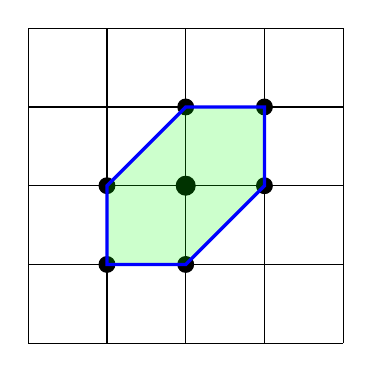
\begin{tikzpicture}
  \draw (0, 0) grid (4, 4); 

\draw [fill=black]  (1, 1) circle (0.1);
\draw [fill=black]  (2, 1) circle (0.1);
\draw [fill=black]  (3, 2) circle (0.1);
\draw [fill=black]  (3, 3) circle (0.1);
\draw [fill=black]  (2, 3) circle (0.1);
\draw [fill=black]  (1, 2) circle (0.1);
\draw [fill=black]  (2, 2) circle (0.12);

\draw [very thick, color=blue, fill=green, fill opacity=0.2]
(1,1) -- (2,1) -- (3,2) -- (3,3) -- (2,3) -- (1,2) -- cycle;

\end{tikzpicture}
\caption{The hexagon, a.k.a the polytope associated to a degree 6 del Pezzo surface.}
\end{figure}
 
Since we have a total of $7$ points in $H \cap N$, the del Pezzo surface is naturally embedded in $\PP^6$. Taking the projective join of two such, we get the (singular) toric variety $T$ in $\PP^{11}$. The polytope associated to this variety is $H \ast H$, the \emph{join} of $H$ with itself. This is obtained by placing each copy of $H$ in disjoint hyperplanes and taking the convex hull. Explicitly, the join of two polytopes $P_1 \subset N_\R$ and $P_2 \subset N_\R$ can be defined in the following way: embed $P_i$ in $N_\R \times N_\R \times \R^2$ as $P_i \times \{e_i\}$. Then take the convex hull of $P_1$ and $P_2$. In our case, we consider the convex hull of the columns of the  matrix

\[
P^\prime = \Conv \left( \left[
\begin{array}{*{14}c}
0 & 1 & 1 & 2 & 2 & 1 & 0 & 0 & 0 & 0 & 0 & 0 & 0 & 0 \\
0 & 0 & 1 & 1 & 2 & 2 & 1 & 0 & 0 & 0 & 0 & 0 & 0 & 0 \\
0 & 0 & 0 & 0 & 0 & 0 & 0 & 0 & 1 & 1 & 2 & 2 & 1 & 0 \\
0 & 0 & 0 & 0 & 0 & 0 & 0 & 0 & 0 & 1 & 1 & 2 & 2 & 1 \\
0 & 0 & 0 & 0 & 0 & 0 & 0 & 1 & 1 & 1 & 1 & 1 & 1 & 1
\end{array} \right] \right)
\]
Note however that $P^\prime$ is not a reflexive polytope anymore. The origin is a vertex, and there are no interior points. This is solved by considering $P := 2 \cdot P^\prime - (1,1,1,1,1)$. This polytope is now reflexive. Since a polytope and any of its multiples have the same normal fan, we can just as well consider $P$ as the polytope associated to $T$.

%In fact: [[[[[ find proof??? ]]]]
%\begin{lemma}
%If $P_1$ and $P_2$ are reflexive polytopes, then $2 \cdot (P_1 \ast P_2)$ is also reflexive.
%\end{lemma}

$P$ lives in $N_\R$, so to get the same setup as in the previous section, we define $\Delta$ to be its polar $P^\circ$. Now $\Delta$ is the convex hull of the columns of the matrix:
\[
\Delta = \Conv \left(
\left[\begin{array}{rrrrrrrrrrrr}
0  & 0  & 0 & 0 & 0 & 0 &  0 & 1 & -1 & 0  & -1 & 1 \\
0  & 0  & 0 & 0 & 0 & 0 &  1 & 0 & 0  & -1 & 1  & -1 \\
0  & -1 & 1 & -1& 0 & 1 &  0 & 0 & 0  & 0  & 0  & 0 \\
-1 & 0  &-1 & 1 & 1 & 0 &  0 & 0 & 0  & 0  & 0  & 0 \\
2  & 2  & 1 & 1 & 1 & 0 &  0 & 0 & -2 & -2 & -1 & -1
\end{array}\right]\right)
\]

Using the program PALP, which is implemented in SAGE, one finds that if one takes $\Delta_1$ (resp. $\Delta_2$) to be convex hull of the first six columns (resp. six last) and the origin, then $\Delta_1+\Delta_2$ is reflexive, which we will, as above, denote by $\nabla^\circ$.

\begin{lemma}
  The $f$-vector of $\nabla^\circ$ is $f=(1, 48, 156, 194, 108, 24, 1)$. 
\end{lemma}

The associated Cayley polytope $P^\ast$ is as above the convex hull of $\Delta_1 \times \{ e_1\}$ and $\Delta_2 \times \{ e_2\} $ in $N_\R \times \R^2$. Explicitly, it is given by the same matrix as $\Delta$, but with $(1,0)$ after the first six columns and $(0,1)$ after the last six.

The Cayley cone $C^\ast$ is just the $7$-dimensional cone supported on $P^\ast$. To find $P$, one just takes the convex hull of the ray generators of $C=(C^\ast)^\ast$. As above, one find $\nabla_1,\nabla_2$ by intersecting with hyperplanes, and then projecting back to $M_\R$. 

\begin{lemma}
$\nabla_1$ and $\nabla_2$ are isomorphic lattice polytopes, differing by a translation in the lattice. In particular, they have the same normal fan.   
\end{lemma}

A calculation in PALP gives the following:
\begin{lemma}
The Hodge numbers associated to this nef partition are $h^{12}=h^{22}=19$ (and consequently, they are the same for the dual nef partition).
\end{lemma}

Here's a summary of the data of all the polytopes found so far:


\begin{center}
  \begin{tabular}{l| c c c c c}
Polytope & Dimension & Lattice points & Interior points & Reflexive & f-vector \\
\hline 
$\Delta$ & $5$ & $15$ & $1$ & Yes & $(12, 48, 74, 48, 12)$ \\
$\Delta^\circ$ & $5$ & $87$ & $1$ & Yes & $(12, 48, 74, 48, 12)$ \\
$\Delta_1$ & $3$ & $8$ & $0$ & No (2) & $(7, 12, 7)$ \\
$\Delta_2$ & $3$ & $8$ & $0$ & No (2) & $(7, 12, 7)$ \\
$\nabla$ & $5$ & $27$ & $1$ & Yes & $(24, 108, 194, 156, 48)$ \\
$\nabla^\circ$ & $5$ & $63$ & $1$ & Yes & $(48, 156, 194, 108, 24)$ \\
$\nabla_1$ & $5$ & $14$ & $0$ & No (2)& $(12, 48, 74, 48, 12)$ \\
$\nabla_2$ & $5$ & $14$ & $0$ & No (2)& $(12, 48, 74, 48, 12)$ \\
\end{tabular} 
\end{center} 
By ``No (2)'' is ment that $2 \cdot P$ is reflexive. 

\section{More - details to arrive}

\begin{itemize}
\item Check all details. In which world do $P$ live?
\item Find explicit description of the nef hypersurfaces.
\item Understand concretely the mirror candidate. 
\item Find subgroup $G$ of $\Aut \K$ acting on $X_t$. Then find subgroup $H$ of $\C^\ast ^n$ acting on the generic element of the family. Mirror candidate is also $\tilde{X_t/H}$. To do this, need to know what kind of singularities $X_t$ has. The group should permute them as well. 
\item Iflg Jan, ``obvious that $\Aut \K$ acts on generic fiber $Y$.
\end{itemize}

\bibliographystyle{alpha} 
\bibliography{bibliografi}

\end{document}
